\subsection{Result Distribution}\label{sec:results_distribution}

Each correlation value in the above graphs is the mean of the correlation
values for 32 benchmark query images with a ground truth ranking of 40 result
images. Calculating the mean correlation per query image for the best
performing configurations shown in \autoref{tab:results_best_performers} shows,
that the retrieval pipelines deal quite well with most image categories
(\autoref{fig:results_distribution}). At the same time the correlation is
almost zero for two of the categories and even significantly below zero for two
more across all pipeline configurations. This suggests that those query images
or image sets have characteristics, that confound the algorithms.
\autoref{fig:results_distribution_outliers} shows the query images with
correlations below zero and examples from the corresponding image set.

\begin{figure}[h]
    \centering
    \pgfplotstableread{results/best_performer_means.csv}\resultsbestperformermeans
\begin{tikzpicture}
    \begin{axis}[
        ybar,
        small,
        width=\textwidth,
        xtick=data,
        xticklabels from table={\resultsbestperformermeans}{key},
        xticklabel style={
            rotate=90,
        },
        extra y ticks= 0,
        extra y tick labels=,
        extra y tick style={grid=major},
        axis x line*=left,
        ymajorgrids,
        error bars/error bar style={
            gray,
        },
        bar width=5pt,
        ]
        \addplot+[error bars/y dir=both, error bars/y explicit] table[x expr=\coordindex, y=mean, y error=stddev]{\resultsbestperformermeans};
    \end{axis}
\end{tikzpicture}
%\pgfplotstableread{results/best_performers.csv}\resultsbestperformers
%\pgfplotstabletranspose*[
    %colnames from=group,
    %columns={group,0.png,1.png,2.png,6.png,7.png,8.png,9.png,10.png,11.png,12.png,13.png,14.png,20.png,21.png,23.png,24.png,25.png,26.png,27.png,28.png,30.png,33.png,34.png,38.png,42.png,43.png,45.png,46.png,47.png,48.png}
%]{\resultsbestperformerstransposed}{\resultsbestperformers}
%\begin{tikzpicture} %[trim axis left, trim axis right]
    %\begin{axis}[
        %ybar=0pt,
        %small,
        %width=\textwidth,
        %xtick=data,
        %xticklabels from table={\resultsbestperformerstransposed}{colnames},
        %xticklabel style={
            %rotate=90,
        %},
        %extra y ticks= 0,
        %extra y tick labels=,
        %extra y tick style={grid=major},
        %axis x line*=left,
        %ymajorgrids,
        %legend style={font=\tiny},
        %legend columns=2,
        %legend pos=south west,
        %vbar/.style={
            %ybar,
            %bar width=1pt,
        %}]
        %\pgfplotsinvokeforeach{1,...,6}{
            %\addplot+[vbar] table[x expr=\coordindex, y index=#1]{\resultsbestperformerstransposed};
            %\pgfplotstablegetcolumnnamebyindex{#1}\of{\resultsbestperformerstransposed}\to{\colname}
            %\addlegendentryexpanded{\colname}
        %}
        %%\addplot+[vbar] table[x expr=\coordindex, y index=2]{\resultsbestperformerstransposed};
    %\end{axis}
%\end{tikzpicture}

    \caption[Distribution of results]{
        The distribution of mean correlations for the configurations of
        \autoref{tab:results_best_performers} shows drastically worse
        performance for some queries.
    }
    \label{fig:results_distribution}
\end{figure}

\begin{figure}[h]
    \centering
    \begin{tabular}{ccc}
        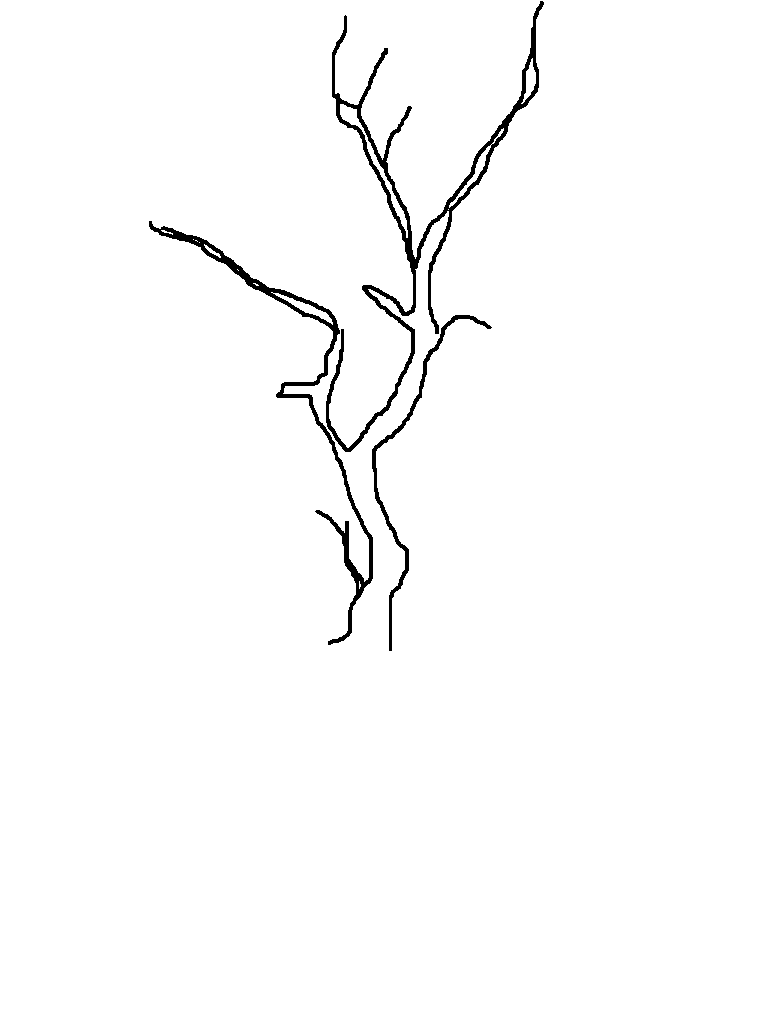
\includegraphics[width=0.3\textwidth,height=2.5cm,keepaspectratio=true]{illustrations/image_examples/sketch_24.png} &
        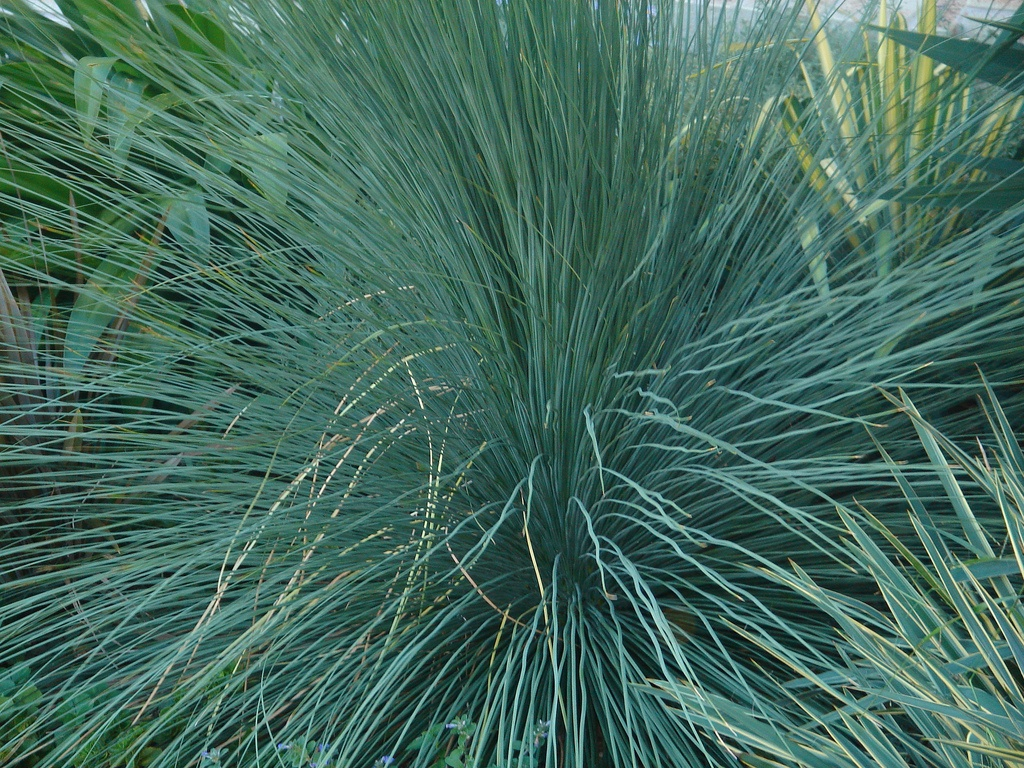
\includegraphics[width=0.3\textwidth,height=2.5cm,keepaspectratio=true]{illustrations/image_examples/result_24_1.jpg} &
        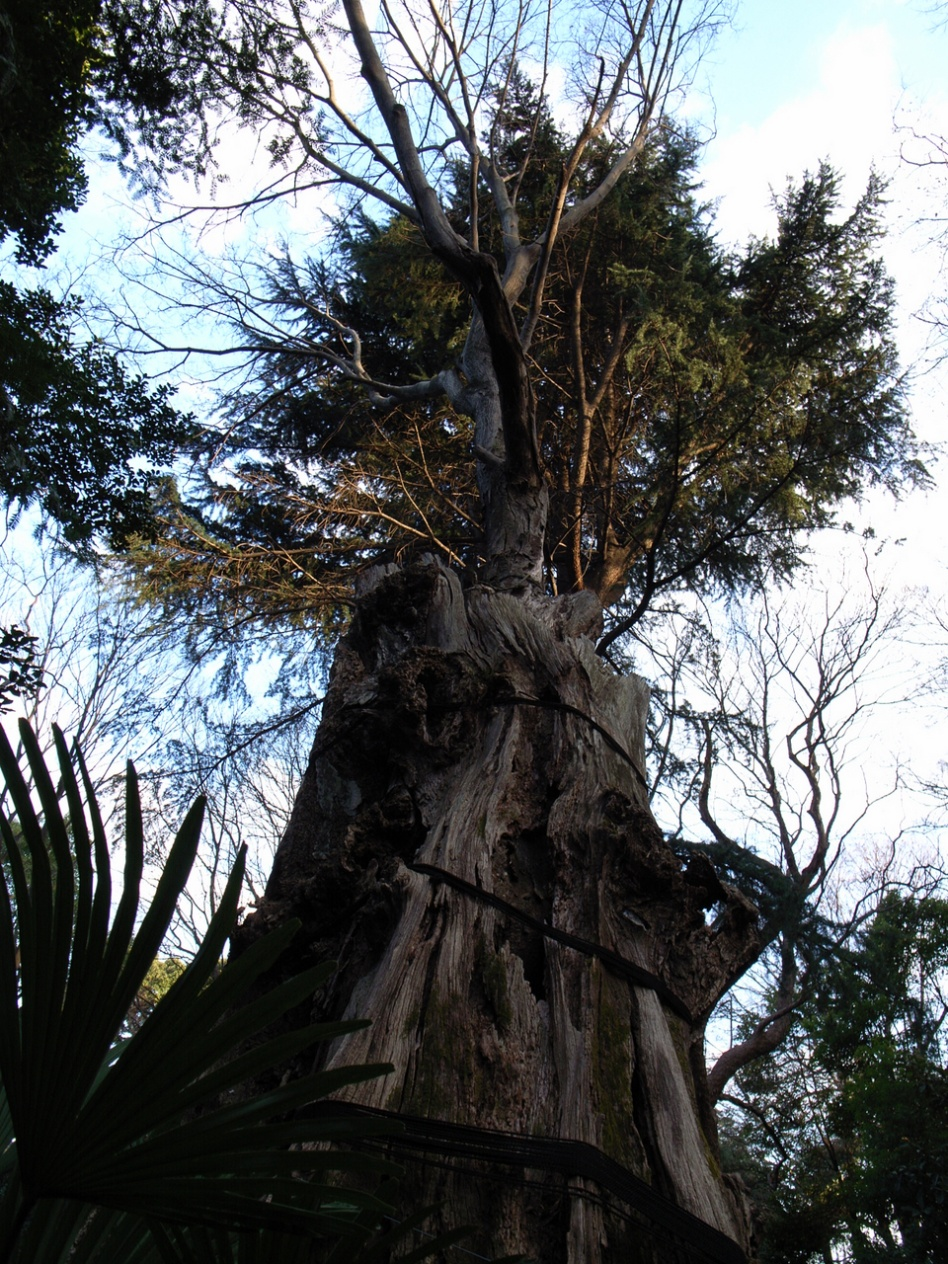
\includegraphics[width=0.3\textwidth,height=2.5cm,keepaspectratio=true]{illustrations/image_examples/result_24_2.jpg} \\
        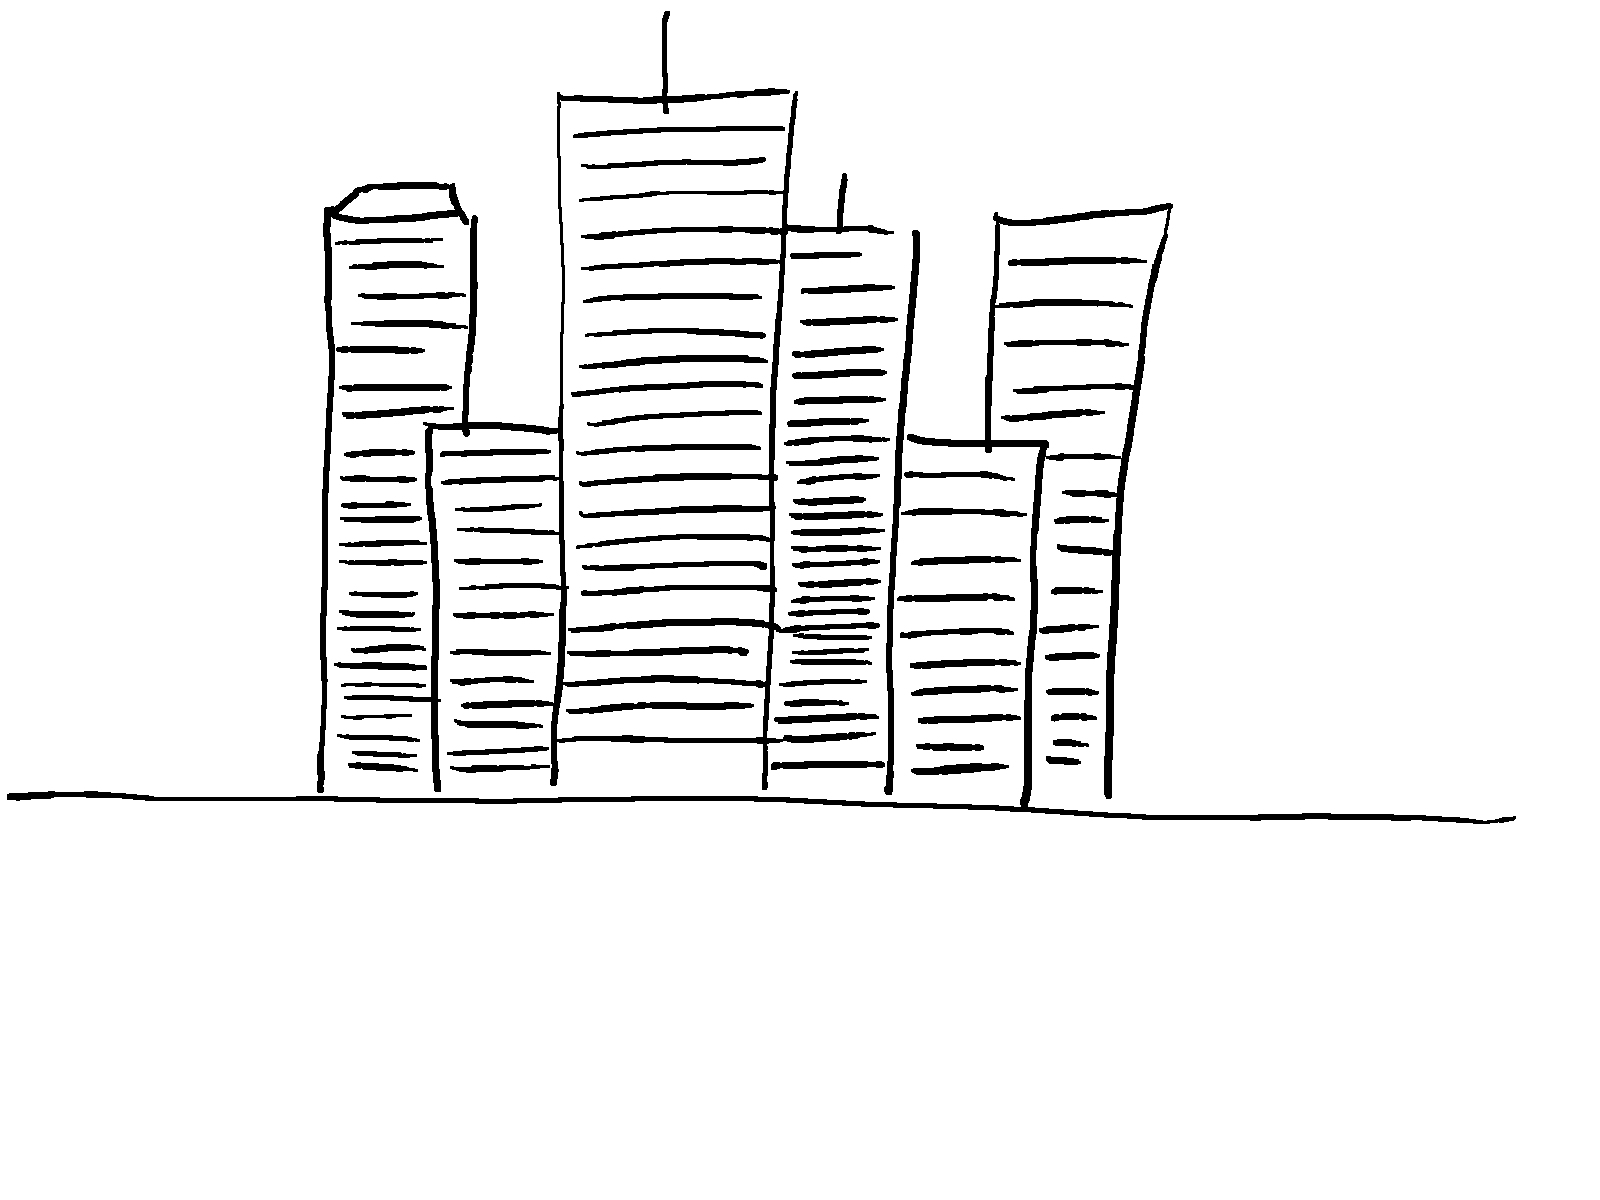
\includegraphics[width=0.3\textwidth,height=2.5cm,keepaspectratio=true]{illustrations/image_examples/sketch_42.png} &
        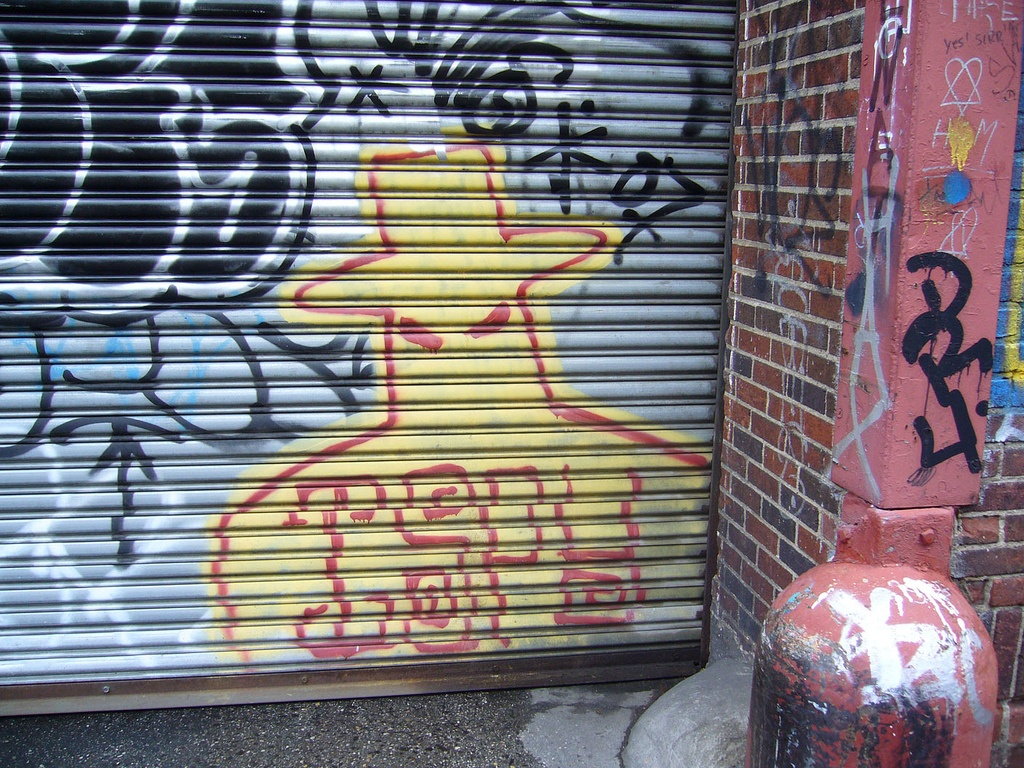
\includegraphics[width=0.3\textwidth,height=2.5cm,keepaspectratio=true]{illustrations/image_examples/result_42_1.jpg} &
        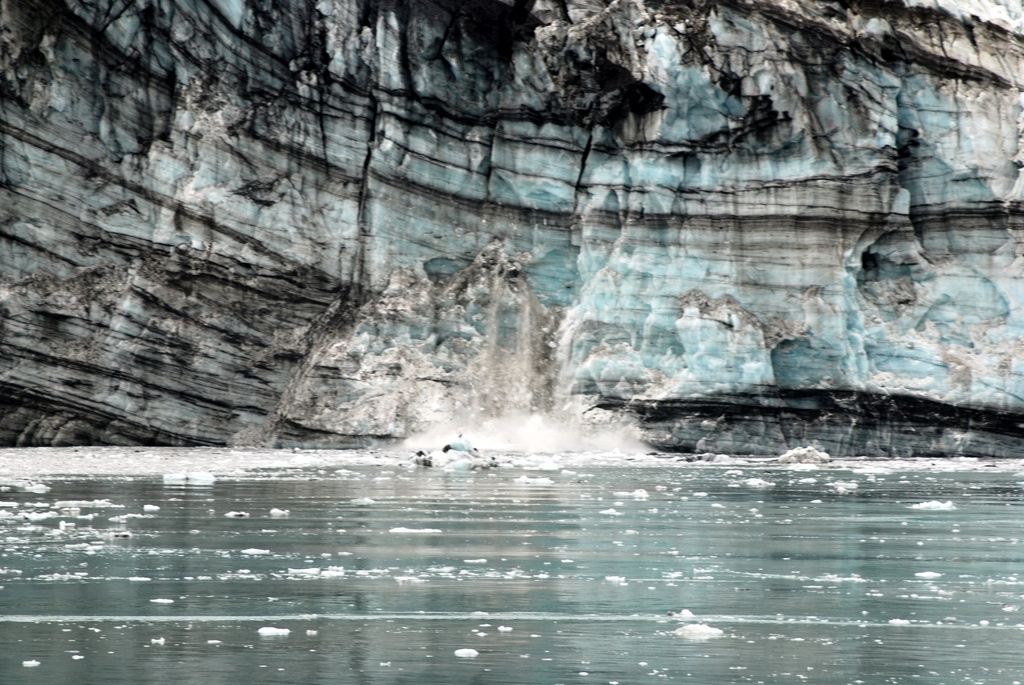
\includegraphics[width=0.3\textwidth,height=2.5cm,keepaspectratio=true]{illustrations/image_examples/result_42_2.jpg}
    \end{tabular}
    \caption[Outlier query images]{
        Outlier query images \texttt{24.png} (top) and \texttt{42.png} (bottom)
        with two example responses.
    }
    \label{fig:results_distribution_outliers}
\end{figure}

\FloatBarrier
